\documentclass[a4paper]{article}

\usepackage[margin=2.5cm]{geometry}
\usepackage[pdftex]{graphicx}
\usepackage[utf8]{inputenc}
\usepackage[T1]{fontenc}
\usepackage{textcomp}
\usepackage{babel}
\usepackage{amsmath, amssymb}
\usepackage[colorlinks=true,linkcolor=blue]{hyperref}
\usepackage{float}
\usepackage{mathrsfs}
%\usepackage{enumitem}
%% for identity function 1:
\usepackage{bbm}
%%For category theory diagrams:
%\usepackage{tikz-cd}
%%For code (e.g. python) in latex:
%\usepackage{listings}
%
%Usage: 
%\begin{lstlisting}[language=Python]
%\end{lstlisting}

\newcommand{\incfig}[2][1]{%
\def\svgwidth{#1\columnwidth}
\import{./figures/}{#2.pdf_tex}
}


% figure support
\usepackage{import}
\usepackage{xifthen}
\pdfminorversion=7
\usepackage{pdfpages}
\usepackage{transparent}

\pdfsuppresswarningpagegroup=1

\setlength\parindent{0pt}

\newcommand{\qed}{\tag*{$\blacksquare$}}
\newcommand{\qedwhite}{\hfill \ensuremath{\Box}}

%Inequalities
\newcommand{\cycsum}{\sum_{\mathrm{cyc}}}
\newcommand{\symsum}{\sum_{\mathrm{sym}}}
\newcommand{\cycprod}{\prod_{\mathrm{cyc}}}
\newcommand{\symprod}{\prod_{\mathrm{sym}}}

%Linear Algebra

\DeclareMathOperator{\Span}{span}
\DeclareMathOperator{\Ima}{Im}
\DeclareMathOperator{\diag}{diag}
\DeclareMathOperator{\Ker}{Ker}
\DeclareMathOperator{\ob}{ob}
\DeclareMathOperator{\Hom}{Hom}
\DeclareMathOperator{\sk}{sk}
\DeclareMathOperator{\Vect}{Vect}
\DeclareMathOperator{\Set}{Set}
\DeclareMathOperator{\Group}{Group}
\DeclareMathOperator{\Ring}{Ring}
\DeclareMathOperator{\Ab}{Ab}
\DeclareMathOperator{\Top}{Top}
\DeclareMathOperator{\Htpy}{Htpy}
\DeclareMathOperator{\Cat}{Cat}
\DeclareMathOperator{\CAT}{CAT}


%Row operations
\newcommand{\elem}[1]{% elementary operations
\xrightarrow{\substack{#1}}%
}

\newcommand{\lelem}[1]{% elementary operations (left alignment)
\xrightarrow{\begin{subarray}{l}#1\end{subarray}}%
}

%SS
\DeclareMathOperator{\supp}{supp}
\DeclareMathOperator{\Var}{Var}

%NT
\DeclareMathOperator{\ord}{ord}

%Alg
\DeclareMathOperator{\Rad}{Rad}
\DeclareMathOperator{\Jac}{Jac}

\DeclareMathAlphabet{\pazocal}{OMS}{zplm}{m}{n}
\newcommand{\unif}{\pazocal{U}}

\begin{document}
    \textbf{p. 91}\\
    \textbf{1:} Let $C$ denote the unit circle in the plane.
    Suppose $f  \colon C \to C$ is a map which is not homotopic to
    the identity. Prove that $f(x) = -x$ for some point 
    $x$ of $C$.\\
    \linebreak
    \textit{Solution:}
    We prove the contrapositive.\\
    Suppose $f(x) \neq -x$ for any point $x$ of $C$. We must show that 
    $f  \colon C \to C$ is homotopic to the identity.\\
    \linebreak
    Since $f(x) \neq -x$ for all $x$, we can define the following map
    $F  \colon C \times I \to C$ by
    \[
       F(s,t) = \frac{s + t \left( f(s) - s \right)     
        }{\| s + t \left( f(s)-s \right) \|}.
    \] 
    It is clear that $F(s,0) = s = \mathbbm{1} (s)$ and
    $F(s,1) = f(s)$, so it remains to show that
    $F(s,t)$ is continuous and well-defined - i.e. that
    $\|s + t \left( f(s) -s \right) \|\neq 0$ for all
    $(s,t) \in C \times I$.\\
    Now, if $s + t \left( f(s) -s \right) = 
    s + t f(s) - ts= 0$ then 
    $\frac{f(s)}{s} = \frac{t-1}{t}$, and since
    $f(s), s \in C$, $\|f(s)\| = 1 = \|s\|$, so
    $\|\frac{t-1}{t}\|= \| \frac{f(s)}{s}\|
    = \frac{\|f(s)\|}{\|s\|} = 1$. Thus since $t \in \mathbb{R}$, we have
    $\frac{t-1}{t} \in \left\{ -1,1 \right\} $. Now
    $\frac{t-1}{t} = 1 \iff -1 = 0$, contradiction. Hence
    $\frac{t-1}{t} = -1$ which implies
    $2t -1 = 0$ so $t = \frac{1}{2}$. Hence
    $ 0 = s + \frac{1}{2} \left( f(s)-s \right) 
    = \frac{f(s)+s}{2}$ which implies
    $f(s) + s = 0$, so $f(s) = -s$ which we assumed not to be the case,
    contradiction. Hence
    $\|s + t\left( f(s) - s \right) \|\neq 0$ for all
    $(s,t) \in C \times I$.\\
    \linebreak
    Now, supposing $C \subset \mathbb{R}^2$, it suffices to
    note for continuity that we must simply check that the
    coordinate functions
    $\pi_i F \to \mathbb{R}, i = 1,2$ are continuous. 
    But writing $s = (s_1, s_2)$ and
    $f(s) = (f_1(s), f_2(s))$, we find that the coordinate functions
    for $s + t \left( f(s) - s \right) $ is
    $s_i + t (f_i(s) - s_i)$ which is continuous as continuous functions are
    stable under sum, difference, product and composition.
    Since $s + t\left( f(s) - s \right) \neq 0$, we find that
    the quotient is continuous too, so $F$ is continuous.\\
    \linebreak

    \textbf{p. 95}\\
    \textbf{13:} Let $G$ be a path-connected topological group.
    Given two loops $\alpha, \beta$ based at $e$ in $G$,
    define a map $F  \colon \left[ 0,1 \right] \times 
    \left[ 0,1 \right]  \to G$ by 
    $F(s,t) = \alpha(s). \beta(t)$ where
    the dot denotes multiplication in $G$. Draw a diagram to show
    the effect of this map on the square, and prove that the
    fundamental group of $G$ is abelian.\\
    \linebreak
    \textit{Solution:} 
    It suffices to show that
    $\pi (G, e)$ is abelian since $G$ is path-connected.\\
    \linebreak
    Let $\langle \alpha \rangle, \langle \beta
    \rangle \in \pi (G, e)$. We want to show that
    $\langle \alpha \rangle * 
    \langle \beta \rangle =\langle \beta \rangle
    * \langle \alpha \rangle$ where $*$ denotes the
    group operation of the fundamental group.\\
    \linebreak
    We must show that
    there is a homotopy
    $\alpha  \beta \simeq \beta  \alpha$, where
    $\alpha \beta$ and $\beta \alpha$ are the usual composition of the paths.\\
    We have
    \[
    \alpha \beta = (\alpha e). (e \beta)
    \simeq (e \alpha). (\beta e)
    = \beta \alpha
    \] 
    since $e \alpha \simeq \alpha e$ and
    $e \beta \simeq \beta e$. Thus
    the fundamental group of $G$ is abelian.
    
   \begin{figure}[H]
       \centering
       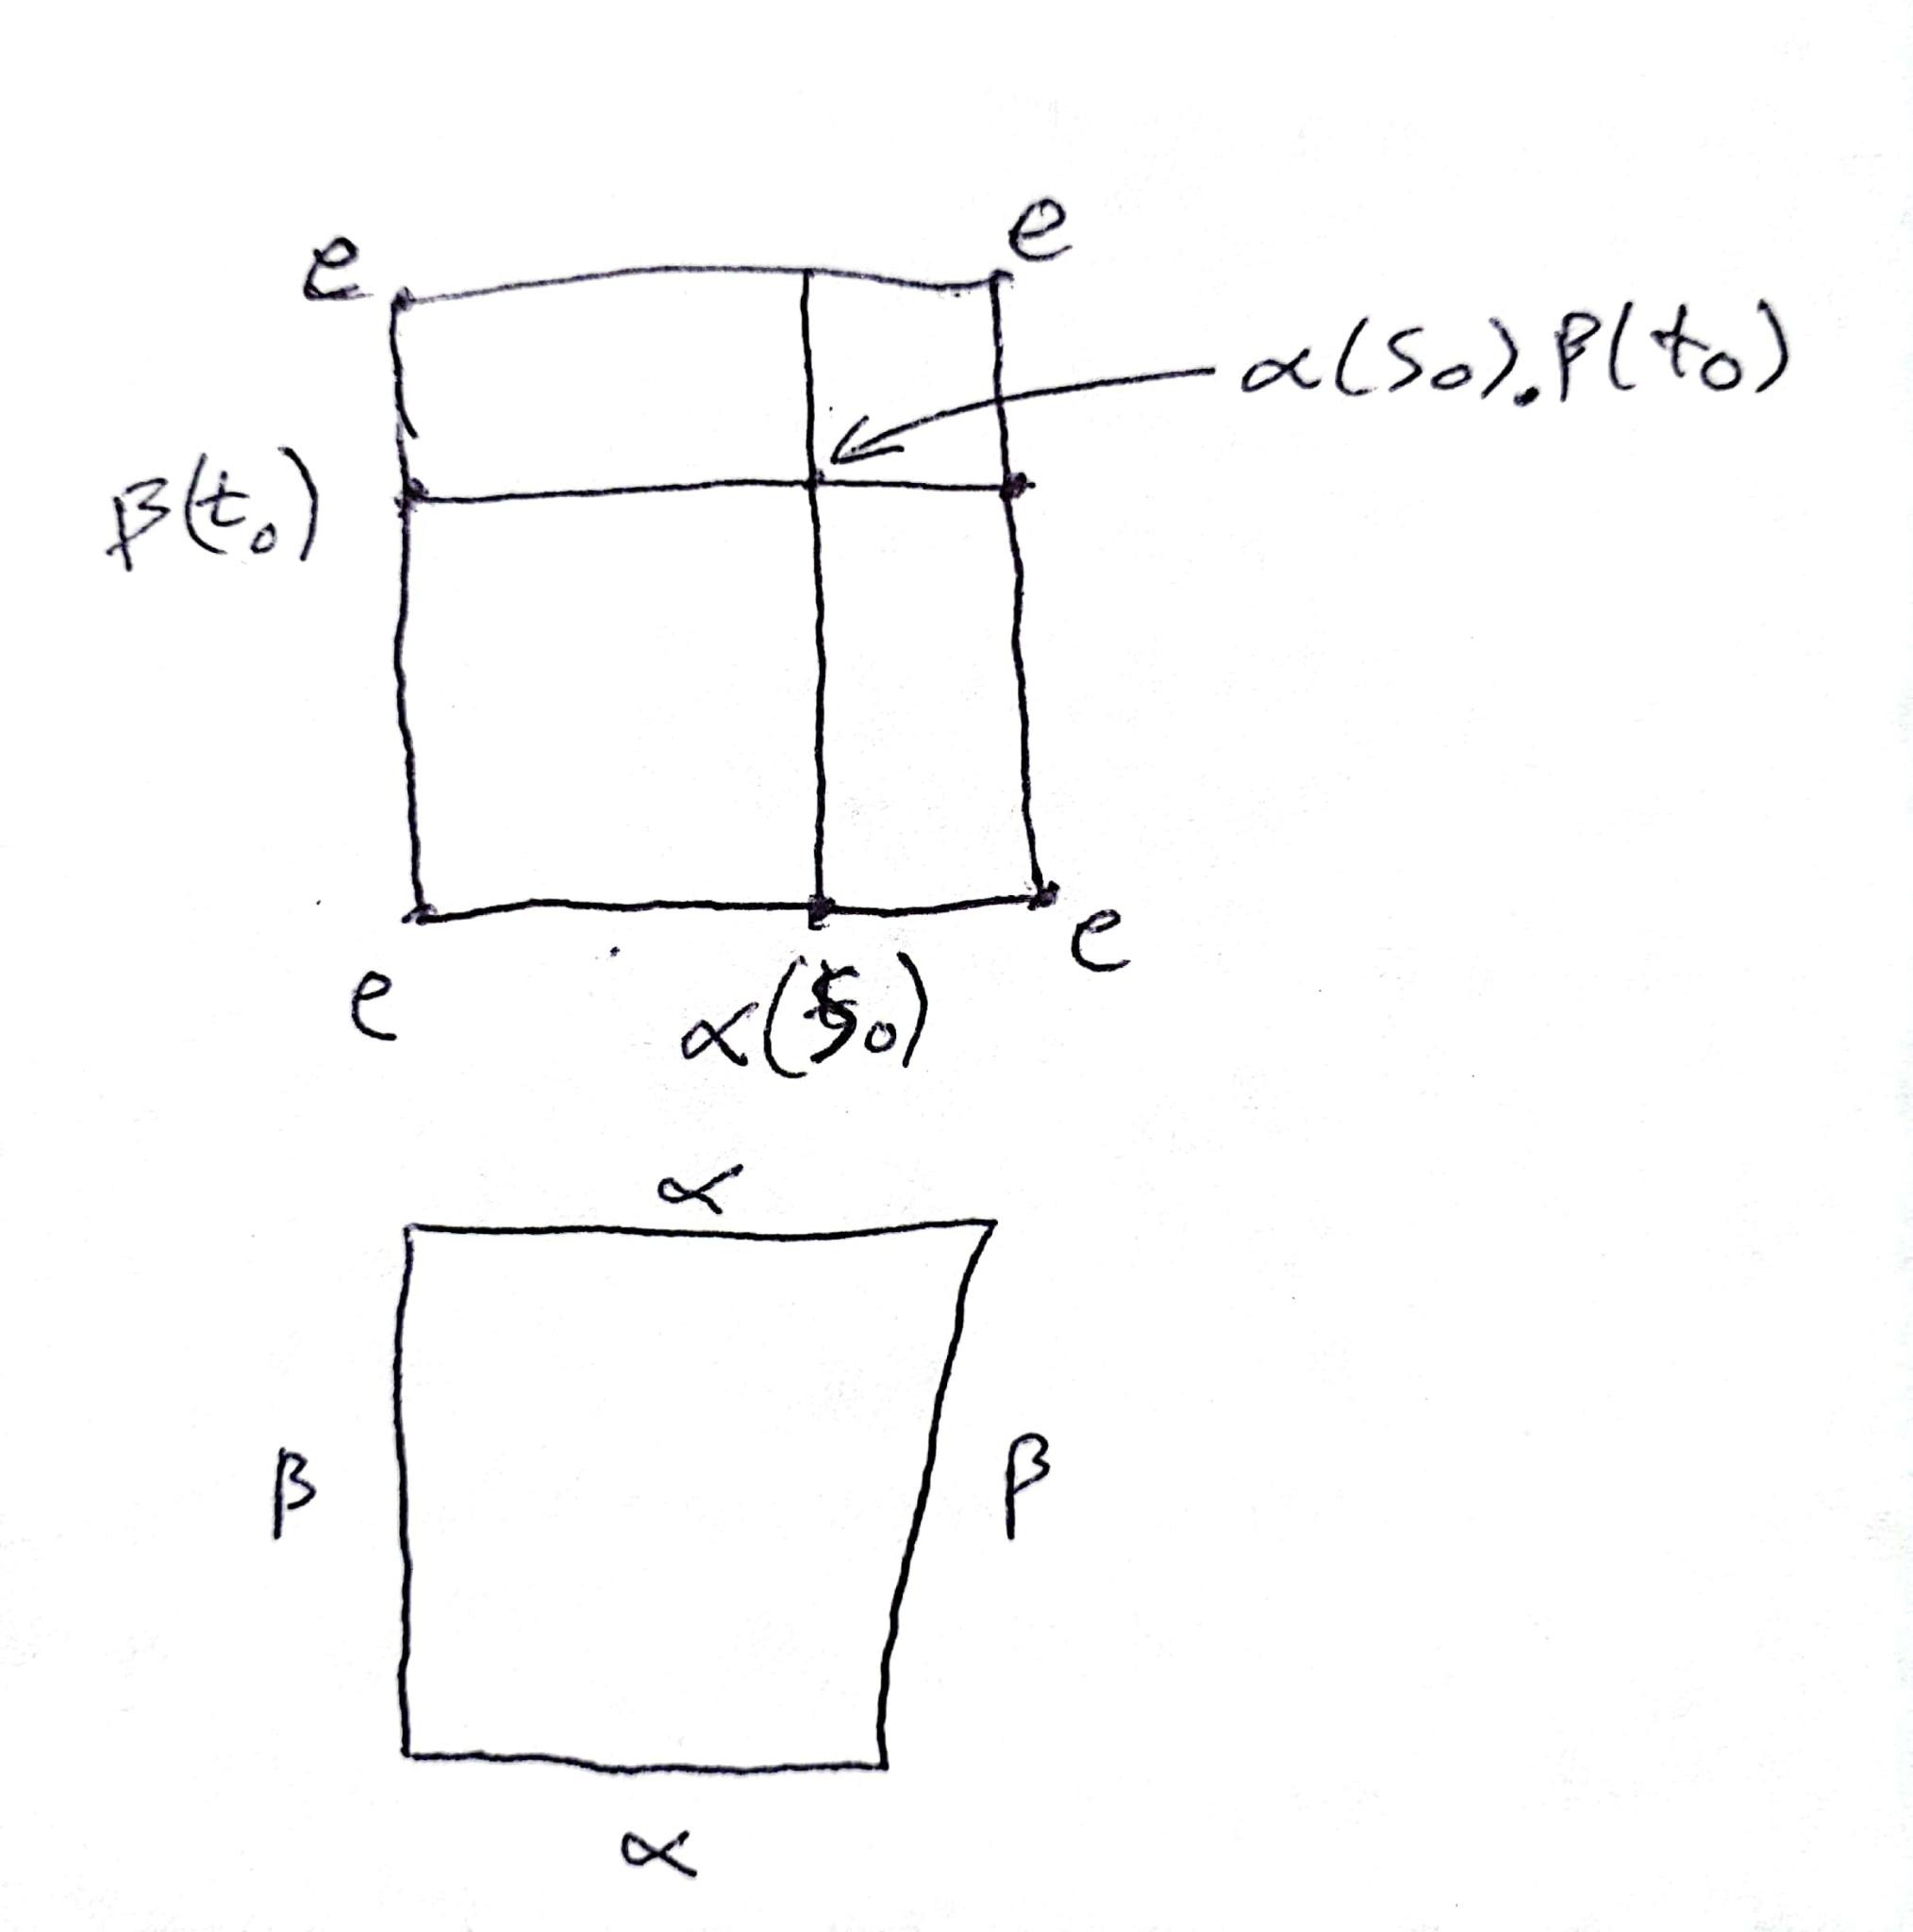
\includegraphics[width=0.6\textwidth]{2.jpeg}
       \label{fig:2-jpeg}
   \end{figure} 




    









































\end{document}
